\documentclass[11pt, dvipsnames, handout]{beamer}
\newtoggle{full}
\settoggle{full}{true}

\newtoggle{covered}
\settoggle{covered}{false}

\newtoggle{presentable}
\settoggle{presentable}{false}

\newtoggle{dualscreen}
\settoggle{dualscreen}{false}

\usepackage{pgfplots}
%\pgfplotsset{compat = newest}

\usepackage{pgfpages}

\setbeamertemplate{note page}{\pagecolor{yellow!5}\vfill \insertnote \vfill}
\usepackage{collect}
\definecollection{notes}
\newcounter{notestaken}

\usepackage{xpatch}

\usepackage{ulem}

\usepackage[framemethod=tikz]{mdframed}

\usepackage{scalerel}
\usepackage{calc}

%\usepackage{enumitem}
\setlength\fboxsep{.2em}

\usepackage{graphicx} % Allows including images
\usepackage{booktabs} % Allows the use of \toprule, \midrule and \bottomrule in tables

\xpatchcmd{\itemize}
  {\def\makelabel}
  {\setlength{\itemsep}{0.65 em}\def\makelabel}
  {}
  {}


\xpatchcmd{\beamer@enum@}
  {\def\makelabel}
  {\setlength{\itemsep}{0.65 em}\def\makelabel}
  {}
  {}


%\makeatletter
%\renewcommand{\itemize}[1][]{%
%  \beamer@ifempty{#1}{}{\def\beamer@defaultospec{#1}}%
%  \ifnum \@itemdepth >2\relax\@toodeep\else
%    \advance\@itemdepth\@ne
%    \beamer@computepref\@itemdepth% sets \beameritemnestingprefix
%    \usebeamerfont{itemize/enumerate \beameritemnestingprefix body}%
%    \usebeamercolor[fg]{itemize/enumerate \beameritemnestingprefix body}%
%    \usebeamertemplate{itemize/enumerate \beameritemnestingprefix body begin}%
%    \list
%      {\usebeamertemplate{itemize \beameritemnestingprefix item}}
%      {%
%        \setlength\topsep{1em}%NEW
%        \setlength\partopsep{1em}%NEW
%        \setlength\itemsep{1em}%NEW
%        \def\makelabel##1{%
%          {%
%            \hss\llap{{%
%                \usebeamerfont*{itemize \beameritemnestingprefix item}%
%                \usebeamercolor[fg]{itemize \beameritemnestingprefix item}##1}}%
%          }%
%        }%
%      }
%  \fi%
%  \beamer@cramped%
%  \raggedright%
%  \beamer@firstlineitemizeunskip%
%}
%
%
%
%
%
%\makeatother

%\setlist[beamer@enum@]{topsep=1 em}
%\let\origcheckmark\checkmark %screw you dingbat
%\let\checkmark\undefined %screw you dingbat
%\usepackage{dingbat} 
%\let\checkmark\origcheckmark %screw you dingbat






%\usepackage{fontawesome}

\usepackage{mathtools}
\usepackage{etoolbox, calculator}

\usepackage{xcolor}
\usepackage{tikz}
\usetikzlibrary{arrows.meta}
\usetikzlibrary{calc}
\usepackage[nomessages]{fp}
\usepackage{transparent}
\usepackage{accsupp}
%\usepackage{color, xcolor}

%colorblind-friendly palette
%\definecolor{dblue}{RGB}{51,34,136}
\definecolor{lblue}{RGB}{136,204,238}
%\definecolor{green}{RGB}{17,119,51}
\definecolor{tan}{RGB}{221,204,119}
%\definecolor{mauve}{RGB}{204,102,119}

\usepackage{tcolorbox}



\usepackage{xifthen}
\usepackage{nicefrac}
\usepackage{amsmath}
\usepackage{amsthm}
\usepackage{amssymb}
\theoremstyle{definition}
\newtheorem*{define}{Definition}
\newtheorem*{recall}{Recall}


\DeclareMathOperator{\tr}{tr}

\usepackage{multicol}
%\setlength{\columnsep}{1cm}

\usepackage{tablists, amsmath,vwcol, cancel, polynom}
\usetikzlibrary{shapes, patterns, decorations.shapes}
%\usepackage{tikzpeople}
\tikzstyle{vertex}=[shape=circle, minimum size=2mm, inner sep=0, fill]
\tikzstyle{opendot}=[shape=circle, minimum size=2mm, inner sep=0, fill=white, draw]

% common math quick commands
\newcommand{\nicedd}[2]{\nicefrac{\text{d}#1}{\text{d}#2}}
\newcommand{\dd}[2]{\dfrac{\text{d}#1}{\text{d}#2}}
\newcommand{\pd}[2]{\dfrac{\partial #1}{\partial#2}}
\renewcommand{\d}[1]{\text{d}#1}
\newcommand{\ddn}[3]{\dfrac{\text{d}^{#3}#1}{\text{d}#2^{#3}}}
\newcommand{\pdn}[3]{\dfrac{\partial^{#3}#1}{\partial#2^{#3}}}
\newcommand{\p}[0]{^{\prime}}
\newcommand{\pp}[0]{^{\prime\prime}}
\newcommand{\op}[2][\text{L}]{#1 \left[ #2 \right]}

\newcommand{\lap}[1]{\mathcal{L}\left\{#1\right\}}
\newcommand{\lapinv}[1]{\mathcal{L}^{-1}\left\{#1\right\}}
\newcommand{\lapint}[1]{\int_0^\infty e^{-st}#1dt}
\newcommand{\evalat}[2]{\Big|_{#1}^{#2}}

\newcommand{\paren}[1]{ \left( #1 \right)}

\newcommand{\haxis}[4][\normcolor]{\draw[#1, <->] (-#2,0)--(#3,0) node[right]{$#4$}; }

\newcommand{\circled}[1]{\raisebox{.5pt}{\textcircled{\raisebox{-.9pt} {#1}}}}
\newcommand{\axis}[4]{\draw[\normcolor, <->] (-#1,0)--(#2,0) 
node[right]{$x$};
\draw[help lines, <->] (0,-#3)--(0,#4) node[above]{$y$};}

\newcommand{\laxis}[6]{\draw[<->] (-#1,0)--(#2,0) 
node[right]{$#5$};
\draw[ <->] (0,-#3)--(0,#4) node[above]{$#6$};}
\newcommand{\xcoord}[2]{
	\draw (#1,.2)--(#1,-.2) node[below]{$#2$};}
\newcommand{\textnode}[3]{
	\draw (#1,#2) node[below]{$#3$};}
	
\newcommand{\nxcoord}[2]{
	\draw (#1,-.2)--(#1,.2) node[above]{$#2$};}
\newcommand{\ycoord}[2]{
	\draw (.2,#1)--(-.2,#1) node[left]{$#2$};}
\newcommand{\nycoord}[2]{
	\draw (-.2,#1)--(.2,#1) node[right]{$#2$};}
\newcommand{\dlim}{\displaystyle\lim}
\newcommand{\dlimx}[1]{\displaystyle\lim_{x \rightarrow #1}}
\newcommand{\stickfig}[2]{
	\draw (#1,#2) arc(-90:270:2mm);
	\draw (#1,#2)--(#1,#2-.5) (#1-.25,#2-.75)--(#1,#2-.5)--(#1+.25,#2-.75) (#1-.2,#2-.2)--(#1+.2,#2-.2);}	

%\newcounter{example}
%\setcounter{example}{1}
%\newcounter{preFrameExample}
%\AtBeginEnvironment{frame}{\setcounter{preFrameExample}{\value{example}}}
%\newcommand{\ex}[1]{
%	 \setcounter{example}{\value{preFrameExample}}
%	 \textcolor{green}{\small\fbox{Example \arabic{example}: #1}}\\[8pt]
%	\stepcounter{example}}
%\newcommand{\exans}[1]{
%	\SUBTRACT{\value{preFrameExample}}{1}{\n}
%	 \textcolor{green}{\small\fbox{Solution \n: #1}}\\[8pt]}
\mode<presentation> {

% The Beamer class comes with a number of default slide themes
% which change the colors and layouts of slides. Below this is a list
% of all the themes, uncomment each in turn to see what they look like.


\usetheme{CambridgeUS}
\usecolortheme[named=black]{structure}


\newcommand{\studentcolor}[0]{ForestGreen}
\newcommand{\normcolor}[0]{NavyBlue}
\newcommand{\alertcolor}{Red}

\setbeamercolor{normal text}{fg=\normcolor}
\setbeamercolor{frametitle}{fg=\normcolor}
\setbeamercolor{section in head/foot}{fg=Black, bg=Gray!20}
\setbeamercolor{subsection in head/foot}{fg=Green!70!Black, bg=Gray!10}
\setbeamercolor{alerted text}{fg=\alertcolor}
\setbeamerfont{alerted text}{series=\bf}
\setbeamertemplate{enumerate items}[default]
\setbeamercolor{enumerate item}{fg=\normcolor}

\setbeamertemplate{footline} % To remove the footer line in all slides uncomment this line
%\setbeamertemplate{footline}[page number] % To replace the footer line in all slides with a simple slide count uncomment this line

\setbeamertemplate{navigation symbols}{} % To remove the navigation symbols from the bottom of all slides uncomment this line
}

\newcommand{\alertbox}[1]{\tcbox[on line, colframe=\alertcolor, colback=White, left=2pt,right=2pt,top=2pt,bottom=2pt]{\usebeamercolor*{normal text}#1}}


\newcommand{\startstu}{\setbeamercolor{normal text}{fg=\studentcolor}\usebeamercolor*{normal text}\setbeamercolor{enumerate item}{fg=\studentcolor}\usebeamercolor*{enumerate item}}
\newcommand{\stopstu}{\setbeamercolor{normal text}{fg=\normcolor}\usebeamercolor*{normal text}\setbeamercolor{enumerate item}{fg=\normcolor}\usebeamercolor*{enumerate item}}

\newcommand{\takenote}[1]{ \begin{collect}{notes}{}{}{}{}  #1  \end{collect}  \addtocounter{notestaken}{1}} %\ifthenelse{\value{notestaken}>0}{\hrulefill\\}{}

\makeatletter
\newcommand{\cover}{\alt{\beamer@makecovered}{\beamer@fakeinvisible}}
\newcommand{\ucover}[1]{\iftoggle{full}{}{\beamer@endcovered} \stopstu #1\startstu \iftoggle{full}{}{\beamer@startcovered} }
%\newcommand{\ucover}[1]{\beamer@endcovered \stopstu #1\startstu \beamer@startcovered }
\makeatother

\newcommand{\skippause}{ \addtocounter{beamerpauses}{-1}}
\newcommand{\blockpres}{ \skippause \pause }

\newcommand{\studentify}[1]{\startstu #1  \stopstu }
\newcommand{\student}[1]{\iftoggle{full}{ \pause  \studentify{#1} }{\iftoggle{covered}{\studentify{#1}}{\cover{  #1 }}}}
\newcommand{\cstudent}[1]{\student{\begin{center} #1 \end{center}}}
\newcommand{\fullonly}[1]{\iftoggle{full}{ #1}{}}
\newcommand{\presentonly}[1]{\iftoggle{presentable}{ #1}{}}

\usepackage{xparse}
\usepackage{xifthen}

% shortcuts for commonly-used presentation elements
%\NewDocumentCommand{\slide}{o m}
% {\IfValueTF{#1}{\begin{frame}[t]{#1}}{\begin{frame}[t]} #2 \end{frame}}

\newtoggle{iscovered}

\newcommand{\slide}[2][]{%
%\setcounter{notestaken}{0}
\takenote{#2} 
%\ifthenelse{\equal{#1}{}}{\begin{frame}[t]}{\begin{frame}[t]{#1}} #2 \ifthenelse{\value{notestaken}>0}{ \note{\includecollection{notes}}}{} \end{frame}%
\ifthenelse{\equal{#1}{}}{\begin{frame}[t]}{\begin{frame}[t]{#1}} #2 \iftoggle{covered}{\settoggle{iscovered}{true}}{\settoggle{iscovered}{false}}  \note{ \iftoggle{iscovered}{}{\settoggle{covered}{true}} #2 \iftoggle{iscovered}{}{\settoggle{covered}{false}} } \end{frame}%
%\setcounter{notestaken}{0}
}
\newcommand{\defn}[2][]{%
 \setcounter{listcounter}{0}%
\ifthenelse{\equal{#1}{}}{\begin{block}{Definition}}{\begin{block}{#1 :}}%
 #2 \vspace{0.25em} \ifthenelse{\value{listcounter}>0}{\skippause}{} \pause \end{block}%
}



\newcommand{\arr}[2]{\begin{array}{#1}#2\end{array}}
\newcommand{\mat}[2]{\left[\arr{#1}{#2}\right]}
\newcommand{\carray}[1]{\arr{c}{#1}}
\newcommand{\larray}[1]{\arr{l}{#1}}
\newcommand{\rarray}[1]{\arr{r}{#1}}
\newcommand{\colvec}[1]{\mat{c}{#1}}

\newcommand{\itmz}[1]{\addtocounter{listcounter}{1} \begin{itemize}#1 \end{itemize} }
\newcommand{\subitem}[1]{\addtocounter{listcounter}{1} \begin{itemize} \item #1 \end{itemize}}
%
\newcommand{\enum}[1]{\addtocounter{listcounter}{1} \begin{enumerate} #1  \end{enumerate}  }


\newcommand{\algnlbl}[1]{\begin{align}#1  \end{align}} 
\newcommand{\algn}[1]{\begin{align*}#1  \end{align*}} 
\newcommand{\lgn}[1]{ \action<+->{#1} }
\newcommand{\slgn}[1]{\iftoggle{full}{\action<+->{ \startstu #1 \stopstu}}{ \cover{ #1 } } \takenote{$#1$}}

\newcommand{\chckmrk}{\alert{\checkmark}}

\usepackage{pifont}
\newcommand{\xmark}{\alert{\text{\large \ding{55}}}}

\newcommand{\return}[0]{\raisebox{.5ex}{\rotatebox[origin=c]{180}{$\Lsh$}}}
\usepackage{pbox}
%\newcommand{\ex}[1]{\rotatebox[origin=c]{10}{\uline{ex}}:$\;$\pbox[t][][b]{0.9\linewidth}{#1}}
\newcommand{\ex}[1]{\uline{ex}:$\;$\pbox[t][][t]{0.9\linewidth}{#1}}
\newcommand{\eg}[1]{e.g.,$\;$\pbox[t][][t]{0.9\linewidth}{#1}}
\newcommand{\tikzplot}[8][]{%
\begin{tikzpicture}

\begin{scope}[]%
\clip(-#2,-#4) rectangle (#3,#5);%
#8%
\end{scope}%
\laxis{#2}{#3}{#4}{#5}{#6}{#7}%
#1
\end{tikzpicture}%
}


\newcommand{\cancelslide}[1]{%
\begingroup%
\setbeamertemplate{background canvas}{%
\begin{tikzpicture}[remember picture,overlay]%
\draw[line width=2pt,red!60!black] %
  (current page.north west) -- (current page.south east);%
\draw[line width=2pt,red!60!black] %
  (current page.south west) -- (current page.north east);%
\end{tikzpicture}}%
#1%
\endgroup%
}
\renewcommand{\CancelColor}{\color{red}}
\newcommand{\twocols}[3][0.5]{\begin{columns}\begin{column}{#1\textwidth}#2\end{column}\hspace{1em}\vrule{}\hspace{1em}\begin{column}{#1\textwidth}#3\end{column}\end{columns}}

\newcommand{\twomini}[5][1]{\calculatespace \begin{minipage}[t]{\columnwidth}\begin{minipage}[][#1\contentheight][t]{#2\columnwidth}#4\end{minipage}\hfill\begin{minipage}[][#1\contentheight][t]{#3\columnwidth}#5\end{minipage}\end{minipage}}

\newcommand{\threemini}[7][1]{\calculatespace \begin{minipage}[t]{\columnwidth}\begin{minipage}[][#1\contentheight][t]{#2\columnwidth}#5\end{minipage}\hfill\begin{minipage}[][#1\contentheight][t]{#4\columnwidth}#6\end{minipage}\hfill\begin{minipage}[][#1\contentheight][t]{#3\columnwidth}#7\end{minipage}\end{minipage}}


\newcounter{listcounter}
\setcounter{listcounter}{0}



\newif\ifsidebartheme
\sidebarthemetrue

\newdimen\contentheight
\newdimen\contentwidth
\newdimen\contentleft
\newdimen\contentbottom
\makeatletter
\newcommand*{\calculatespace}{%
\contentheight=\paperheight%
\ifx\beamer@frametitle\@empty%
    \setbox\@tempboxa=\box\voidb@x%
  \else%
    \setbox\@tempboxa=\vbox{%
      \vbox{}%
      {\parskip0pt\usebeamertemplate***{frametitle}}%
    }%
    \ifsidebartheme%
      \advance\contentheight by-1em%
    \fi%
  \fi%
\advance\contentheight by-\ht\@tempboxa%
\advance\contentheight by-\dp\@tempboxa%
\advance\contentheight by-\beamer@frametopskip%
\ifbeamer@plainframe%
\contentbottom=0pt%
\else%
\advance\contentheight by-\headheight%
\advance\contentheight by\headdp%
\advance\contentheight by-\footheight%
\advance\contentheight by4pt%
\contentbottom=\footheight%
\advance\contentbottom by-4pt%
\fi%
\contentwidth=\paperwidth%
\ifbeamer@plainframe%
\contentleft=0pt%
\else%
\advance\contentwidth by-\beamer@rightsidebar%
\advance\contentwidth by-\beamer@leftsidebar\relax%
\contentleft=\beamer@leftsidebar%
\fi%
}
\makeatother


\iftoggle{dualscreen}{\setbeameroption{show notes on second screen=right}}{}

\usepackage{gensymb}
\begin{document}

\section{Lecture 27}

\subsection{Wave Equation}
\slide[Waves travelling on strings \hfill  \hspace{2em}\begin{minipage}{0.25\textwidth}{ 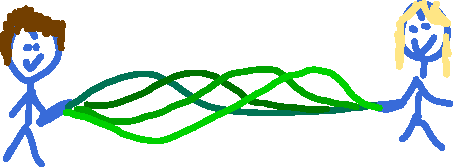
\includegraphics[height=1.25cm]{images/wavekids.pdf}}\end{minipage}  ]{
\vfill
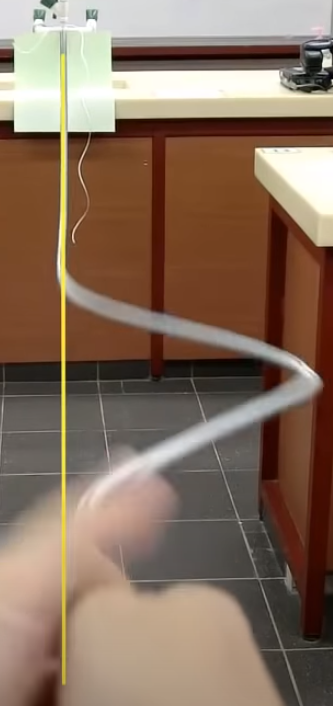
\includegraphics[height=4.5cm]{images/wave_1.png}\hfill
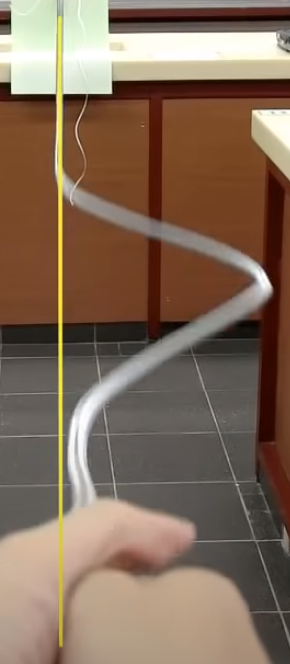
\includegraphics[height=4.5cm]{images/wave_2.png}\hfill
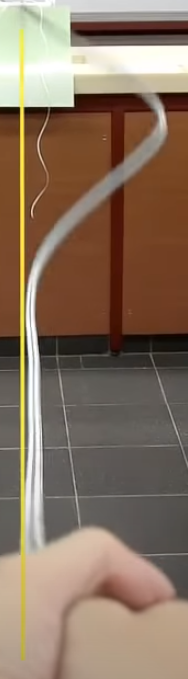
\includegraphics[height=4.5cm]{images/wave_3.png}\hfill
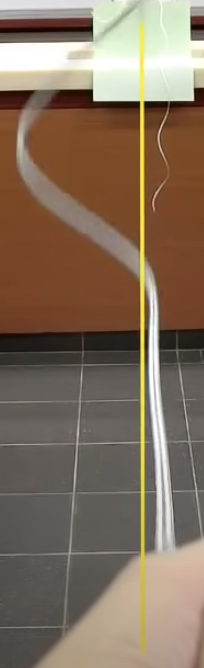
\includegraphics[height=4.5cm]{images/wave_4.png}\hfill
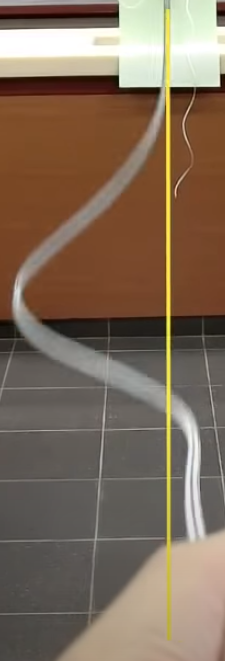
\includegraphics[height=4.5cm]{images/wave_5.png}\hfill\\
\small  source: \url{https://www.youtube.com/watch?v=PVX4V5Adbzk}
\vfill
guitar strings: \url{https://vine.co/v/Oqx7BJgazKZ}
}

\slide[Wave Equation: $y_{tt}=c^2y_{xx}$]{
\uline{Plucked string under tension:} $c^2=\frac{T}{\rho}$ 
\itmz{ \item $T=$tension
\item $\rho=$mass density of the string (mass/length)}
\vfill
\centerline{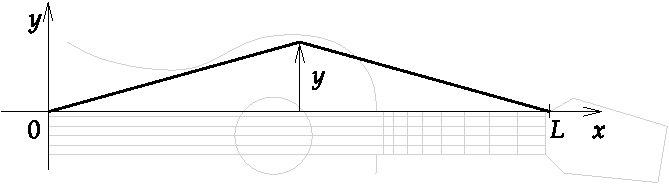
\includegraphics[width=10cm]{images/sps-vibstr-tex4ht.pdf}}
\vfill
\uline{Tapped elastic rod:} $c^2=\frac{E}{\rho}$ \\
\itmz{\item $E=$Young's Modulus
\item $\rho=$mass density of the rod (mass/length)}
}

\slide[Boundary Conditions and Initial Conditions: $y_{tt}=c^2y_{xx}$]{
\centerline{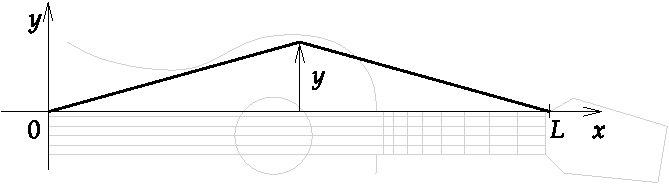
\includegraphics[width=10cm]{images/sps-vibstr-tex4ht.pdf}}
Boundary Conditions:
\student{
Clamped end-points\[y(0)=y(L)=0\]}\vfill
Initial Conditions:\vfill
\student{Now we need two, because of the two time derivatives\algn{y(x,0)&=f(x)\\y_t(x,0)&=g(x)}}
\vfill
}
\subsection{Superposition}
\slide[The Wave Equation is Homogeneous: Superposition]{\vspace{-1em}
Suppose we find two solutions to the wave equation $w(x,t)$ and $z(x,t)$, then a linear combination \[y(x,t)=c_1w(x,t)+c_2z(x,t)\] is also a solution.
\vfill
Proof:
\student{
We are given 
\[ w_{tt} = c^2w_{xx}\qquad \uline{\text{and}} \qquad z_{tt} = c^2z_{xx} \]
with \[w(0)=w(L)=0 \qquad \uline{\text{and}} \qquad  z(0)=z(L)=0 \]
then 
\algn{y_{tt}&=c_1 w_{tt}+c_2z_{tt} =c_1 c^2w_{xx} + c_2 c^2 z_{xx}\\
&=c^2y_{xx}}
with 
\[y(0)=c_1w(0)+c_2z(0)=0 \qquad \uline{\text{and}} \qquad y(L)=c_1w(L)+c_2z(L)=0 \]
}
}

\slide[Decomposition into two simpler problems: Superposition]{
\centerline{ $y_{tt}=c^2y_{xx}, \quad y(0)=y(L)=0, \quad  y(x,0)=f(x), \quad y_t(x,0)=g(x)$}
\[y(x,t) = w(x,t) + z(x,t)\]
Problem 1: initial velocity, but no displacement of string
\student{\algn{w_{tt}&=c^2 w_{xx} & w(x,0)&=0  \\ w(0,t)&=w(L,t)=0&
w_t(x,0)&=g(x) \qquad \text{for } 0<x<L
}}
\vspace{.25em}

Problem 2: initial displacement, but no velocity of string
\student{\algn{z_{tt}&=c^2 z_{xx} & z(x,0)&= f(x) \qquad \text{for } 0<x<L\\z(0,t)&=z(L,t)=0 & z_t(x,0)&=0
}
\vfill
\centerline{Solve each problem by separation of variables}
}
}


\slide[Separation of Variables: Problem 1]{\vspace{-2em}
\algn{w_{tt}&=c^2 w_{xx} & w(x,0)&=0  \\ w(0,t)&=w(L,t)=0&
w_t(x,0)&=g(x) \qquad \text{for } 0<x<L
}
Try $w(x,t)=X(x)T(t)$
\student{\algn{\frac{T\pp(t)}{c^2T(t)} &= \frac{X\pp(x)}{X(x)} =-\lambda \\
\text{BCs}\Rightarrow X_n(x)&= b_n\sin\left( \frac{n\pi}{L}x\right)\\
T_n(t)&=A_n \cos\left( \frac{n\pi c}{L}t\right) + B_n \sin\left( \frac{n\pi c}{L}t\right)\\\\
w(x,0)=0 \quad \Rightarrow \quad A_n &= 0\\
\text{arbitrarily choose } B_n &= \frac{L}{n\pi c} \qquad \Rightarrow T_n\p(0) = 1 
 }
}
}

\slide[Separation of Variables + Superposition: Problem 1]{\vspace{-3em}
\algn{w_{tt}&=c^2 w_{xx} & w(x,0)&=0  \\ w(0,t)&=w(L,t)=0&
w_t(x,0)&=g(x) \qquad \text{for } 0<x<L
}
with $w_n(x,t)=\frac{L}{n\pi c} \sin\left( \frac{n\pi c}{L}t\right) b_n\sin\left( \frac{n\pi}{L}x\right) $
\student{\hfill $w(x,t) = \sum_{n=1}^\infty w_n(x,t)$ \hfill~ \algn{ \intertext{Initial condition: } w_t(x,0) &= \sum_{n=1}^\infty T_n'(0) b_n \sin\left( \frac{n\pi}{L}x\right)=\sum_{n=1}^\infty  b_n \sin\left( \frac{n\pi}{L}x\right) =  g(x)
 }\vfill
use an odd periodic extension of $g(x)$: \hfill $b_n = \frac{2}{L}\intop_0^L g(x) \sin\paren{\frac{n\pi}{L}x}$ \hfill ~
\vfill
\[w(x,t) = \sum_{n=1}^\infty \frac{L}{n\pi c} \sin\left( \frac{n\pi c}{L}t\right) b_n\sin\left( \frac{n\pi}{L}x\right) \]
}
}

\slide[Separation of Variables: Problem 2]{\vspace{-2em}
\algn{z_{tt}&=c^2 z_{xx} & z(x,0)&= f(x) \qquad \text{for } 0<x<L\\z(0,t)&=z(L,t)=0 & z_t(x,0)&=0
}
Try $z(x,t)=X(x)T(t)$
\student{\algn{\frac{T\pp(t)}{c^2T(t)} &= \frac{X\pp(x)}{X(x)} =-\lambda \\
\text{BCs}\Rightarrow X_n(x)&= c_n\sin\left( \frac{n\pi}{L}x\right)\\
T_n(t)&=A_n \cos\left( \frac{n\pi c}{L}t\right) + B_n \sin\left( \frac{n\pi c}{L}t\right)\\\\
z_t(x,0)=0 \quad \Rightarrow \quad B_n &= 0\\
\text{arbitrarily choose } A_n &=1 \qquad \Rightarrow T_n(0) = 1 
 }
}
}

\slide[Separation of Variables + Superposition: Problem 2]{\vspace{-3em}
\algn{z_{tt}&=c^2 z_{xx} & z(x,0)&= f(x) \qquad \text{for } 0<x<L\\z(0,t)&=z(L,t)=0 & z_t(x,0)&=0
}
with $z_n(x,t)= \cos\left( \frac{n\pi c}{L}t\right) c_n\sin\left( \frac{n\pi}{L}x\right) $
\student{\hfill $z(x,t) = \sum_{n=1}^\infty z_n(x,t) $ \hfill ~ \algn{\intertext{Initial condition: } z(x,0) = f(x) &= \sum_{n=1}^\infty c_n \sin\left( \frac{n\pi}{L}x\right)
 }\vfill
use an odd periodic extension of $f(x)$: $c_n = \frac{2}{L}\intop_0^L f(x) \sin\paren{\frac{n\pi}{L}x}$
\vfill
\[z(x,t) = \sum_{n=1}^\infty \cos\left( \frac{n\pi c}{L}t\right) c_n\sin\left( \frac{n\pi}{L}x\right) \]
}
}

\slide[Fourier Solution to the Wave Equation]{
\centerline{ $y_{tt}=c^2y_{xx}, \quad y(0)=y(L)=0, \quad  y(x,0)=f(x), \quad y_t(x,0)=g(x)$}
\vfill
\algn{y(x,t) &= w(x,t) + z(x,t)\\&=\sum_{n=1}^\infty \sin\left( \frac{n\pi}{L}x\right) \left[ b_n \frac{L}{n\pi c} \sin\left( \frac{n\pi c}{L}t\right)  + c_n \cos\left( \frac{n\pi c}{L}t\right)  \right] }\vfill
$c_n$ is obtained from an odd periodic extension of $f(x)$\\ \vspace{.25em}\centerline{$c_n = \frac{2}{L}\intop_0^L f(x) \sin\paren{\frac{n\pi}{L}x}$}\vfill
$b_n$ is obtained from an odd periodic extension of $g(x)$\\ \vspace{.25em}\centerline{$b_n = \frac{2}{L}\intop_0^L g(x) \sin\paren{\frac{n\pi}{L}x}$}
}
\end{document}